\DiaryEntry{Exponential Distribution, 2}{2019-09-06}{Stochastic}

Previously, we considered two RVs with exponential distribution (and different rates) and showed that the distribution of their maximum is \emph{not} exponential (the minimum is). Furthermore, we showed that if the rates are very different, the distribution of the maximum can be approximated by the exponential distributioh with samaller rate (at least for large values).

Here we want to consider what happens if we take the maximum of $N$ RVs each with the same exponential distribution; 

\bee
X = \max_i X_i, \quad X_i \sim \text{Exp}(\lambda), \quad k=1,\ldots,N
\eee

By the results from \ref{2019-08-30:entry}, we have for the cdf

\bee
P(X < t) = \left( 1 - e^{-\lambda t}\right)^N
\eee

and the pdf can be obtained as

\bee
f_X(t) = \frac{dP(X<t)}{dt} = \lambda N e^{-\lambda t}\left( 1 - e^{-\lambda t}\right)^{N-1}
\eee

The following Figure shows the pdf of $X_1$ (blue), and the pdfs of $X$ for $N=5$ (red) and $N=10$ (green), respectively (for $\lambda = 1/2$).

\begin{figure}[hbt!]
\centering
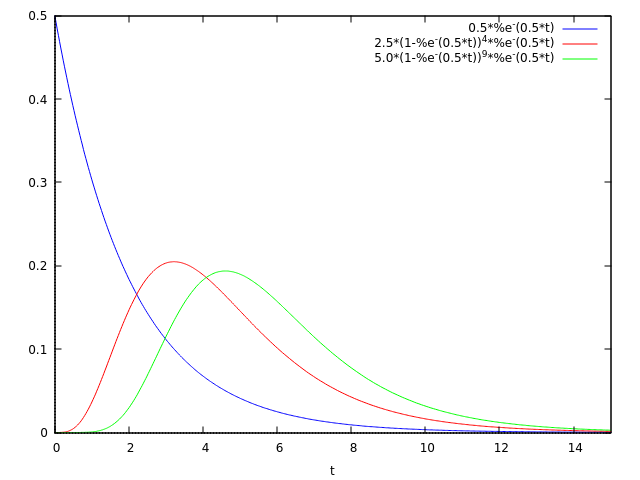
\includegraphics[scale=0.7]{images/exp_pdf_2_1.png}
\end{figure}

Larger values of $N$ move the maximum of the pdf to the right; Maxima (see \href{files/2019-09-06-exponential_pdf_3.wxmx}{file}) indicates that the position $t^\star$ of the maximum follows

\bee
t^\star = \frac{\log N}{\lambda}
\eee

We can calculate the location of the minimumby standard methods; we have

\bee
\frac{d f_X(t)}{dt} = \lambda N (-\lambda) e^{-\lambda t} \left(1 - e^{-\lambda t} \right)^{N-1} + \lambda N e^{-\lambda t} (-\lambda) \left( - e^{-\lambda t} \right) (N-1) \left(1 - e^{-\lambda t} \right)^{N-2}
\eee

Setting this to zero and simplifying yields

\bee
\frac{d f_X(t)}{dt} = (N-1) e^{-\lambda t} - \left(1 - e^{-\lambda t} \right) = 0
\eee

and we further obtain

\bee
e^{-\lambda t} \left[N-1+1\right]-1 = 0
\eee

and from this follows

\bee
t^\star = \frac{\log N}{\lambda}
\eee

as location for the maximum. \qed

%%% Local Variables:
%%% mode: latex
%%% TeX-master: "journal"
%%% End:
